\documentclass[11pt]{report}
\usepackage{tikz}
\usetikzlibrary{fit,positioning}

\begin{document}
\begin{titlepage}
\begin{figure}
\centering
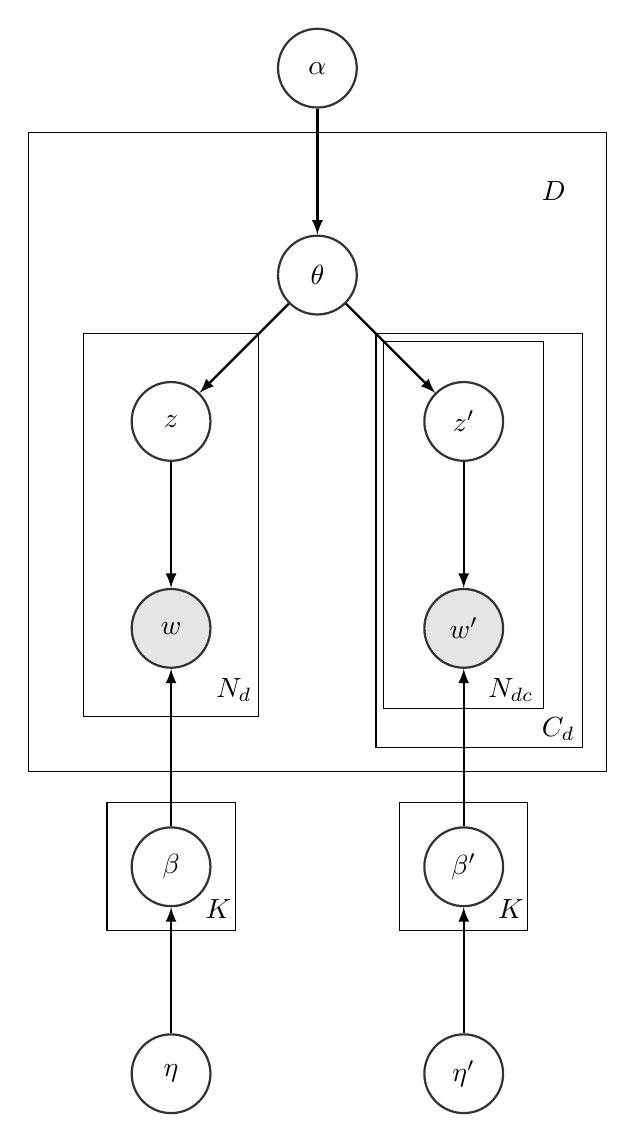
\begin{tikzpicture}
\tikzstyle{main}=[circle, minimum size = 10mm, thick, draw =black!80, node distance = 16mm]
\tikzstyle{connect}=[-latex, thick]
\tikzstyle{box}=[rectangle, draw=black!100]
  \node[main] (alpha) [label=center:$\alpha$] {};
  \node[main] (theta) [below=of alpha,label=center:$\theta$]{};
  \node[main] (z) [below left=of theta,label=center:$z$]{};
  \node[main, fill = black!10] (w) [below =of z,label=center:$w$]{};
  \node[main] (beta) [below = 20mm of w,label=center:$\beta$]{};
  \node[main] (eta) [below =of beta,label=center:$\eta$]{};
  
  \node[main] (z') [below right=of theta,label=center:$z'$]{};
  \node[main, fill = black!10] (w') [below=of z',label=center:$w'$]{};
  \node[main] (beta') [below = 20mm of w', label=center:$\beta'$]{};
  \node[main] (eta') [below = of beta', label=center:$\eta'$]{};
  
  \path (alpha) edge [connect] (theta)
  	(theta) edge [connect] (z)
	(z) edge [connect] (w)
	(eta) edge [connect] (beta)
	(beta) edge [connect] (w)	
	(theta) edge [connect] (z')
	(z') edge [connect] (w')
	(eta') edge [connect] (beta')
	(beta') edge [connect] (w');

  \node[rectangle] (articles) [inner sep=13mm, draw=black!100, fit = (theta) (z) (w) (z') (w'), label= {[shift={(3.0,-1.0)}] $D$}] {};
  \node[rectangle, inner sep=6mm, draw=black!100, fit = (z) (w), label={[shift={(0.8, -4.8)}] $N_d$}] {};
  \node[rectangle, inner sep=8mm, draw=black!100, fit = (z') (w'), label={[shift={(1, -5.3)}] $C_d$}, xshift=2mm, yshift=-2mm]{};
  \node[rectangle, inner sep=5mm, draw=black!100, fit = (z') (w'), label={[shift={(.6, -4.7)}] $N_{dc}$}]{};
  \node[rectangle, inner sep=3mm, draw = black!100, fit= (beta), label={[shift={(0.6, -1.6)}] $K$}]{};
  \node[rectangle, inner sep=3mm, draw=black!100, fit = (beta'), label={[shift={(0.6, -1.6)}] $K$}]{};
\end{tikzpicture}
\end{figure}
\end{titlepage}

\end{document}